\section{Module 2: Lecture 6\\The Fourier Transform}

\subsection{Introduction}
We are now in a position where we can deal with more general signals from the point of view of decomposition into sinusoidal frequency components and analysis as to what happens when you pass them through a linear shift invariant system. To do that, let's recapitulate some of the important conclusions that we had drawn in the previous chapter which will now help us in generalization.
%%%
%%%
\subsection{Recapitulation}
Let $\mathbb{S}$ be a linear shift invariant system with impulse response $h(t)$, and to it, we give a periodic signal input. Let’s assume that the Dirichlet conditions are obeyed. So we could decompose this into its Fourier series.
\begin{equation*}
x(t)= \sum\limits_{k=-\infty}^{k=+\infty}c(k)e^{j\Omega kt}
\end{equation*}
Where $\Omega=2\pi /T$ is the angular frequency and $c(k)$ are the Fourier coefficients. Now, the output can also be written as a Fourier series.
\begin{equation*}
y(t)= \sum\limits_{k=-\infty}^{k=+\infty}c(k)H(k\Omega)e^{j\Omega kt}
\end{equation*}
where
\begin{equation*}
H(\Omega)= \int_{-\infty}^{+\infty} \! h(t)e^{-j\Omega t} \ \dm t
\end{equation*}
%%%
%%%
\subsection{Interpretation of $H(\Omega)$ as a Dot Product}
We can interpret $H(\Omega)$ as a dot product or inner product. It’s an inner product between the impulse response $h(t)$ and the rotating phasor $e^{j\Omega t}$. An inner product with a unit vector calculates the projection or a component of the vector along the unit vector. So it's as if we are trying to find the component of the impulse response along a rotating phasor, rotating with an angular velocity $\Omega$. And, at the specific values of $\Omega$ given by each of the Fourier series components, we evaluate this dot product and use it to modify the Fourier series coefficient.
We can see from the equation of output $y(t)$ that output Fourier series coefficients are $c(k)H(\Omega k)$. Recall that in the input, the Fourier series coefficients were calculated by taking an inner product taking only one period of the input for the integral.
We took only one period of the input, and found the inner product with the corresponding harmonic or the complex exponential rotating with that particular multiple of the fundamental frequency. This is how we calculate the Fourier series coefficients.\\
Now, we can see that the Fourier coefficients of the output are the \emph{component by component multiplication of the Fourier coefficients of the input and impulse response}.
\[
Y(k\Omega)= c(k)H(k\Omega)
\]
Now, there are two questions to answer here. Here we have assumed that the input was periodic. What if it is not? Can we generalize this to a non-periodic function is a question that we need to answer. Secondly, can we think of this quantity $H(\Omega)$ as a new transform or a new way of dealing with the impulse response in its own right?\\
Now, a transform will make sense or will be adequate only if it is invertible. That is to say, we should be able to get back $h(t)$ from $H(\Omega)$. There should be no loss of information. It turns out that this is indeed the case. We can call $H(\Omega)$, for any $\Omega \in \mathbb{R}$, as the \emph{Fourier transform} of the impulse response $h(t)$.\\
Now let's try to address the question as to how can we \emph{go back} to $h(t)$ from $H(\Omega)$.
%%%
%%%
\subsection{Inverse for the Fourier Transform}
The answer to the question again lies in vector intuition. As we have seen, $H(\Omega)$ is the component of $h(t)$ along the phasor $e^{j\Omega t}$ for all such $\Omega \in \mathbb{R}$. In vector algebra, we get back a vector from its components by multiplying the components with their corresponding unit vectors and summing them. So, if $\hat{u}_1$ and $\hat{u}_2$ are two orthogonal unit vectors in two dimensions, $\overrightarrow{v}$ is a 2-D vector, and
\[
\langle \overrightarrow{v},\hat{u}_1 \rangle = v_1, \langle \overrightarrow{v},\hat{u}_2 \rangle = v_2
\]
Then, we construct $\overrightarrow{v}$ by multiplying the components with the corresponding unit vector and summing them. Hence
\[
\overrightarrow{v} = v_1\hat{u}_1 + v_2\hat{u}_2
\]
Now using the same principle here, $H(\Omega)$ are the components of the ``vector'' $h(t)$ along the unit vectors $e^{j\Omega t}$. Hence, to obtain the vector $h(t)$ back, we should multiply the component by the unit vector and sum up, or in this case, integrate over all $\Omega$.\\
But there are two subtleties involved here. Firstly, we don't know whether in this vector space of integrable functions, the vector $e^{j\Omega t}$ is a unit vector or not. That is, whether its magnitude is one or not. In case it is not one, we have to multiply it by a suitable constant to make it a unit vector. Secondly, we don't know whether $e^{j\Omega_1 t}$ and $e^{j\Omega_2 t}$ are orthogonal or not, for $\Omega_1 \neq \Omega_2$.\\
In the following subsection, we proceed to evaluate the inverse of $H(\Omega)$ assuming two things; one is that the vectors $e^{j\Omega t}$ are orthogonal, and that the multiplying factor $\kappa_0$ (for making it a unit vector) is independent of $\Omega$.
%%%
%%%
\subsubsection{Finding the Inverse of the Fourier Transform}
Form the previous discussion, the quantity we propose to be the inverse of $H(\Omega)$ is given by
\[
I = \int_{-\infty}^{\infty} \! H(\Omega)\ \kappa_0 e^{j\Omega t} \ \dm \Omega
\]
Now, we know that
\[
H(\Omega)= \int_{-\infty}^{\infty} \! h(t_1)e^{-j\Omega t_1} \ \dm t_1
\]
Putting this in $I$, we get,
\[
I = \int_{-\infty}^{\infty} \! \int_{-\infty}^{\infty} \! h(t_1)e^{-j\Omega t_1}\ \dm t_1 \ \kappa_0 e^{j\Omega t} \ \dm \Omega
\]
\[
= \int_{-\infty}^{\infty} \! h(t_1) \left\lbrace \int_{-\infty}^{\infty} \! \kappa_0 e^{-j\Omega t_1} \  e^{j\Omega t} \ \dm \Omega \right\rbrace \dm t_1
\]
Let's evaluate the quantity in the braces. We can write it as
\[
\lim_{\Omega_1 \to \infty} \int_{-\Omega_1}^{+\Omega_1} \! \kappa_0 e^{j\Omega (t-t_1)} \ \mathrm{d}\Omega
\]

\[
= \lim_{\Omega_1 \to \infty} \kappa_0 \frac{e^{j\Omega_1 (t-t_1)}-e^{-j\Omega (t-t_1)}}{j(t-t_1)}
\]

\[
= \lim_{\Omega_1 \to \infty}\frac{2\kappa_0 j\sin(\Omega_1 (t-t_1))}{j(t-t_1)}
\]

\[
= \lim_{\Omega_1 \to \infty}\frac{2\kappa_0\Omega_1\sin(\Omega_1 (t-t_1))}{\Omega_1(t-t_1)}
\]

Now, this can be written as 
\[
\lim_{\Omega_1 \to \infty} 2\kappa_0\Omega_1 \frac{\sin(x)}{x}
\]
where $x=\Omega_1(t-t_1)$. Now, $\sin(x)/x$ is not defined at $x=0$ as it has a zero divided by zero form. So we evaluate the limit as $x\to 0$.
\[
\lim_{x \to 0}\frac{\sin(x)}{x} = \lim_{x \to 0}\frac{\cos(x)}{1} = 1
\]
where the first equality is due to L'H\^opital's rule. This function will be oscillatory due to $\sin(x)$, but will decay as $x$ increases, due to the $x$ in the denominator. Also, the function will be zero when $x=n\pi$ or $\Omega_1(t-t_1)=n\pi$. Now, let's deal with this function as a function of $(t-t_1)$ rather than $x$. Let us try to plot the function
\[
f(t-t_1) = \frac{2\kappa_0\Omega_1\sin(\Omega_1 (t-t_1))}{\Omega_1(t-t_1)}
\]
The value of $\sin(x)/x$ is $1$ as $x \to 0$ as we saw earlier. Hence $f(0)=2\kappa_0\Omega_1$. Also the first null of the function will occur at $\Omega_1(t-t_1)=\pi$ or $(t-t_1)=\pi/\Omega_1$. Also the function is even with respect to $(t-t_1)$.
\begin{figure}[ht]
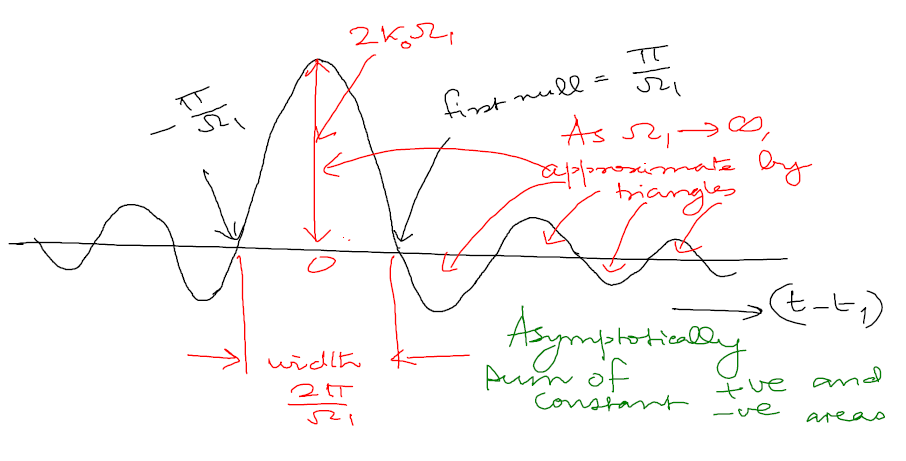
\includegraphics[scale=0.6]{fig.png}
\label{fig:sinc}
\caption{Sinc function}
\end{figure}
Hence, we will get a plot roughly as shown in Fig.\ref{fig:sinc}.
Now, we have to look at what happens when $\Omega_1 \to \infty$. We can see that the height of the main lobe at $x=0$ goes to infinity, but the width of the lobe, which is $2\pi/\Omega_1$ goes to zero, as $\Omega_1 \to \infty$. It can also be shown that the area of the other smaller lobes add up to zero, due to their alternating nature. Hence, we have a \emph{pulse} whose height is tending to infinity and the width to zero. In that case, we can assume the central lobe to be a triangle. Hence its area will be
\[
A = \frac{1}{2}\frac{2\pi}{\Omega_1}2\kappa_0\Omega_1 = 2\pi\kappa_0
\]
Hence, we can see that this area is a constant independent of $\Omega_1$. So we have a pulse having infinite magnitude and zero width, with a constant area encapsulated by it, and as you will remember from Part 1, this is nothing but the \emph{impulse function} $2\pi\kappa_0\delta(t-t_1)$.\\
Now, going back to our integral $I$,
\[
I = \int_{-\infty}^{\infty} \! h(t_1) \left\lbrace \int_{-\infty}^{+\infty} \! \kappa_0 e^{-j\Omega t_1} \  e^{j\Omega t} \ \mathrm{d}\Omega \right\rbrace \mathrm{d}t_1
\]
And we have evaluated the quantity in the braces to be $2\pi\kappa_0\delta(t-t_1)$. Hence,
\[
I = \int_{-\infty}^{\infty} \! h(t_1)\left\lbrace 2\pi\kappa_0\delta(t-t_1) \right\rbrace \mathrm{d}t_1 = 2\pi\kappa_0 \int_{-\infty}^{\infty} \! h(t_1) \delta(t-t_1)\ \mathrm{d}t_1
\]
Hence, by the sifting property of the delta function, we have,
\[
I = 2\pi\kappa_0 h(t)
\]
Hence, we can now set the value of $\kappa_0$ such that $I = h(t)$ as required. Hence $\kappa_0 = 1/2\pi$.\\
Hence, we finally have our expression for the \emph{Inverse Fourier transform} of $H(\Omega)$.
\[
h(t) = \frac{1}{2\pi}\int_{-\infty}^{\infty} \! H(\Omega)\  e^{j\Omega t} \ \mathrm{d}\Omega
\]
%%%
%%%
\subsection{Orthogonality of the Complex Exponentials}
A valid question to ask here is where did the orthogonality of the complex exponentials come in the picture. The answer lies in the integral in the braces which we evaluated.
\[
\int_{-\infty}^{+\infty} \! \kappa_0 e^{-j\Omega t_1} \  e^{j\Omega t} \ \mathrm{d}\Omega = 2\pi\kappa_0 \delta(t-t_1)
\]
or,
\[
\int_{-\infty}^{+\infty} \! e^{j\Omega t} \ \overline{e^{j\Omega t_1}} \ \mathrm{d}\Omega = 2\pi \delta(t-t_1)
\]
where the bar indicates complex conjugate. Now, this can be also written by renaming the variables, treating $t$ as the independent variable, as
\[
\int_{-\infty}^{+\infty} \! e^{j\Omega_1 t} \ \overline{e^{j\Omega_2 t}} \ \mathrm{d}t = 2\pi \delta(\Omega_1-\Omega_2)
\]
Now, we can immediately see that this is like an inner product between phasors rotating with different frequencies $\Omega_1$ and $\Omega_2$, and what this statement says is that it is non zero only for $\Omega_1=\Omega_2$. Hence, we do have some sense of orthogonality here. But since the value is infinite when the frequencies are equal, we have to call this a generalized orthogonality relation.
%%%
%%%
\subsection {Implications} 
Let's try to find what the Fourier transform expression implies. We have a non-periodic function $h(t)$ and we have decomposed it in its Fourier coefficients, not for discrete, but continuous set of frequency values, from minus to plus infinity. This can be thought of in the following way: We think of a non-periodic function as a periodic function with period tending to infinity. This is a valid statement, because as a periodic with period $T$ repeats itself after an interval $T$, we can say that a non-periodic function repeats itself after $T \to \infty$. Now, as the time period increases, the spacing between two adjacent frequencies decreases. And
\[
f = \lim_{T\to\infty}\frac{2\pi}{T} = 0.
\]
Hence, for a non-periodic function, the spacing between the adjacent frequencies tends to zero, which amounts to the Fourier spectrum going to continuous from discrete. This is exactly what has happened. The Fourier transform $H(\Omega)$ is a continuous function, and in general has a non-zero value for all $\Omega \in \mathbb{R}$.





